\uuid{tFtI}
\exo7id{5721}
\auteur{rouget}
\organisation{exo7}
\datecreate{2010-10-16}
\isIndication{false}
\isCorrection{true}
\chapitre{Calcul d'intégrales}
\sousChapitre{Intégrale impropre}

\contenu{
\texte{
Etude complète de $f~:~x\mapsto\int_{x}^{x^2}\frac{1}{\ln t}\;dt$.
}
\reponse{
\textbullet~\textbf{Domaine de définition.} Soit $x\in\Rr$.

Si $x < 0$, la fonction $t\mapsto\frac{1}{\ln t}$  n'est pas définie sur $[x,0[\subset[x,x^2]$ et $f(x)$ n'est pas défini.

Si $0< x < 1$, $[x^2,x]\subset]0,1[$. Donc la fonction $t\mapsto\frac{1}{\ln t}$ est continue sur $[x^2,x]$. Dans ce cas, $f(x)$ existe et est de plus strictement positif car $\ln t < 0$ pour tout $t$ de $]0,1[$.
 

Si $x > 1$, $[x,x^2]\subset]1,+\infty[$. Donc la fonction $t\mapsto\frac{1}{\ln t}$ est continue sur $[x,x^2]$. Dans ce cas aussi, $f(x)$ existe et est strictement positif.

Enfin, $f(0)$ et $f(1)$ n'ont pas de sens.

\begin{center}
\shadowbox{
$f$ est définie sur $D =]0,1[\cup]1,+\infty[$ et strictement positive sur $D$.
}
\end{center}

 \textbullet~\textbf{Dérivabilité.} Soit $I$ l'un des deux intervalles $]0,1[$ ou $]1,+\infty[$. La fonction $t\mapsto\frac{1}{\ln t}$ est continue sur $I$. Soit $F$ une primitive de cette fonction sur $I$.
 
Si $x\in]0,1[$, on a $[x^2,x]\subset]0,1[$ et donc $f(x)=F(x^2)-F(x)$. De même, si $x\in]1,+\infty[$.

On en déduit que $f$ est de classe $C^1$ sur $D$. De plus, pour $x\in D$, 

\begin{center}
$f'(x) =2xF'(x^2) - F'(x) =\frac{2x}{\ln(x^2)}-\frac{1}{\ln x}=\frac{x-1}{\ln x}$.
\end{center}

\textbullet~\textbf{Variations.} $f'$ est strictement positive sur $]0,1[\cup]1,+\infty[$ et donc $f$ est strictement croissante sur $]0,1[$ et sur $]1,+\infty[$ (mais pas nécessairement sur $D$).
 
 

 \textbullet~\textbf{Etude en $0$.}
Soit $x\in]0,1[$. On a $0<x^2 < x < 1$ et de plus la fonction $t\mapsto\frac{1}{\ln t}$ est décroissante sur $[x^2,x]\subset]0,1[$ en tant qu'inverse d'une fonction strictement négative et strictement croissante sur $]0,1[$. Donc, $\frac{x-x^2}{\ln x}\leqslant\int_{x^2}^{x}\frac{1}{\ln t}\;dt\leqslant\frac{x-x^2}{\ln(x^2)}$ puis

\begin{center}
$\forall x\in]0,1[$,  $\frac{x^2-x}{2\ln x}\leqslant f(x)\leqslant\frac{x^2-x}{\ln x}$.
\end{center}

On en déduit que $\lim_{x \rightarrow 0^+}f(x) = 0$ et on peut prolonger $f$ par continuité en $0$ en posant $f(0) = 0$ (on note encore $f$ le prolongement).

Quand $x$ tend vers $0$ par valeurs supérieures, $f'(x) =\frac{x-1}{\ln x}$  tend vers 0. Ainsi,

- $f$ est continue sur $[0,1[$,

- $f$ est de classe $C^1$ sur $]0,1[$,

- $f'$ a une limite réelle quand $x$ tend vers $0$ à savoir $0$.

D'après un théorème classique d'analyse, $f$ est de classe $C^1$ sur $[0,1[$ et $f'(0) = 0$.

 \textbullet~\textbf{Etude en 1.} On a vu à l'exercice \ref{ex:rou7bis} que $\lim_{x \rightarrow 1}f(x)=\ln2$ (la limite à droite en $1$ se traite de manière analogue). On prolonge $f$ par continuité en $1$ en posant $f(1) =\ln2$ (on note encore $f$ le prolongement obtenu).
 

Ensuite quand $x$ tend vers $1$, $f'(x)$ tend vers $1$. Donc $f$ est de classe $C^1$ sur $\Rr^+$ et $f'(1)=1$.

En particulier, $f$ est continue sur $\Rr^+$ et d'après plus haut f est strictement croissante sur $\Rr^+$.

 \textbullet~\textbf{Etude en $+\infty$.} Pour  $x > 1$, $f(x)\geqslant{x^2-x}{\ln x}$. Donc $f(x)$ et $\frac{f(x)}{x}$ tendent vers $+\infty$  quand $x$ tend vers $+\infty$.
La courbe représentative de $f$ admet en $+\infty$ une branche parabolique de direction $(Oy)$.

 \textbullet~\textbf{Convexité.} Pour $x\in D$, $f''(x)=\frac{\ln x-\frac{x-1}{x}}{\ln^2x}$.
 

En $1$, en posant $x = 1+h$ où $h$ tend vers $0$, on obtient

\begin{center}
$f''(1+h)=\frac{(1+h)\ln(1+h)-h}{(1+h)\ln^2(1+h)}=\frac{(1+h)\left(h-\frac{h^2}{2}+o(h^2)\right)-h}{h^2+o(h^2)}=\frac{1}{2}+o(1)$.
\end{center}

$f$ est donc de classe $C^2$ sur $]0,+\infty[$ et $f''(1) =\frac{1}{2}$.

Pour $x\neq 1$, $f''(x)$  est du signe de $g(x)=\ln x - 1 +\frac{1}{x}$ dont la dérivée est $g'(x)=\frac{1}{x}-\frac{1}{x^2}=\frac{x-1}{x^2}$. La fonction $g$ est stictement décroissante sur $]0,1]$ et strictement croissante sur $[1,+\infty[$. Donc pour $x\neq1$, $g(x)> g(1) = 0$. On en déduit que pour tout $x\in]0,+\infty[$, $f''(x) > 0$ et donc que $f$ est strictement convexe sur $\Rr^+$.

\textbullet~\textbf{Graphe.}

$$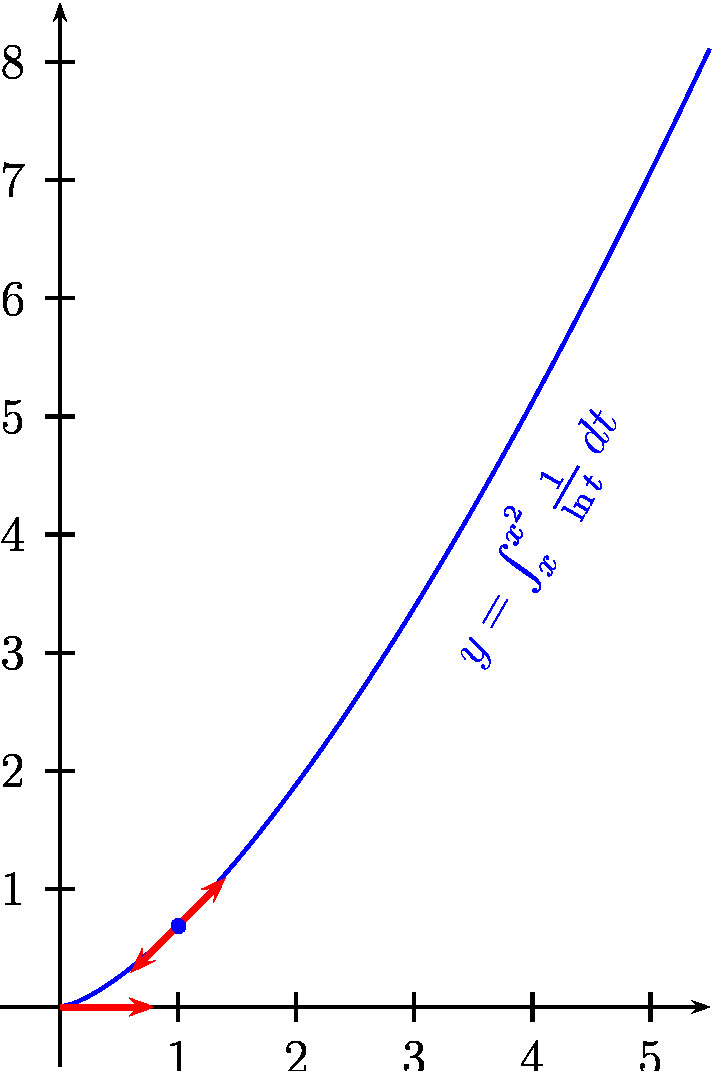
\includegraphics{../images/img005721-1}$$
}
}
